\documentclass[conference]{IEEEtran}
\IEEEoverridecommandlockouts

\usepackage{cite}
\usepackage{amsmath,amssymb}
\usepackage{graphicx}
\usepackage{booktabs}
\usepackage{array}
\usepackage{multirow}
\usepackage{tikz}
\usepackage{pgfplots}
\pgfplotsset{compat=1.18}
\usetikzlibrary{arrows.meta,positioning,fit}

\begin{document}

\title{A Bilingual Voice-Driven Conversational Assistant for\\Accessible E-Commerce Interfaces}

\author{
\IEEEauthorblockN{Muhammad Mateen Amjad\IEEEauthorrefmark{1},
                  Abdullah Zahid\IEEEauthorrefmark{2},
                  Hoor ul Ain Amir\IEEEauthorrefmark{3}}
\IEEEauthorblockA{Department of Computer Engineering,
Information Technology University (ITU), Lahore, Pakistan\\
\IEEEauthorrefmark{1}BSCE22005 \quad
\IEEEauthorrefmark{2}BSCE22040 \quad
\IEEEauthorrefmark{3}BSCE22037}
}

\maketitle

% ================================================================
% ABSTRACT
% ================================================================
\begin{abstract}
E-commerce interfaces in Pakistan are predominantly designed around
typed English queries, dense visual navigation, and menu-based purchase
flows, creating barriers for Urdu-dominant users, older adults, and
low-literacy populations. This paper presents VoiceBazaar, a bilingual
multimodal HCI prototype for voice-driven product search, cart
management, and order confirmation. The system combines browser-based
automatic speech recognition, a text-input fallback, a bilingual
rule-based natural language understanding (NLU) engine, visual product
results, and conversational feedback supporting English, Roman Urdu,
Urdu script, and code-switched commands. A 17-item product catalogue
and a 25-command evaluation set spanning six intent classes and four
language modes were used to measure intent recognition and slot
extraction. The system achieved 100\% intent accuracy, 100\%
category-slot accuracy, 100\% color-slot accuracy, and 100\% exact
command match on the scripted evaluation set. Results show that a
lightweight bilingual rule-based NLU pipeline can support end-to-end
voice shopping tasks while exposing key limitations in vocabulary
coverage, speech recognition reliability, and handling of open-domain
product synonyms. The contribution includes an accessible voice-first
e-commerce interaction design, a fully evaluated MERN prototype, and
design implications for multilingual conversational commerce in
low-resource language settings.
\end{abstract}

\begin{IEEEkeywords}
human-computer interaction, voice user interface, bilingual assistant,
Urdu NLP, conversational commerce, accessibility
\end{IEEEkeywords}

% ================================================================
% 1. INTRODUCTION
% ================================================================
\section{Introduction}

Human-computer interaction has evolved from single-modality desktop
input toward interfaces that combine speech, text, touch, visual
feedback, and AI-mediated dialogue~\cite{mctear2016rise}. Multimodal
systems are especially important where conventional interfaces impose
literacy, language, or motor barriers. In Pakistan, mainstream
e-commerce platforms expect users to type product names in English,
parse English-only labels, and navigate visually dense category trees.
This design creates significant friction for the country's
predominantly Urdu-speaking population, older adults, low-literacy
users, and users with motor or visual impairments.

Voice interaction can reduce these barriers because speech is a natural
communication channel, yet current commercial voice assistants continue
to underperform for multilingual and code-switched users~%
\cite{choi2023multilingual,kann2022plurilingualism}. For e-commerce
specifically, the problem is compounded: a system must distinguish
exploratory browsing from high-stakes transactional intent, maintain
cart context across turns, recover from recognition errors, and elicit
explicit confirmation before committing an order~%
\cite{radlinski2017conversational,zamora2017dave}. Prior work on voice
shopping~\cite{rhee2020voice}, multilingual assistants~%
\cite{zhang2021language}, and Urdu automatic speech
recognition~\cite{arif2025wer,sharif2024urdu} shows steady progress,
but few systems address a complete English--Urdu conversational
shopping workflow with accessible HCI principles.

The main contributions of this paper are:
\begin{itemize}
  \item A working multimodal MERN prototype (VoiceBazaar) for bilingual
        voice-driven product search, cart management, and order
        confirmation.
  \item A lightweight English, Roman Urdu, Urdu script, and
        code-switched NLU pipeline evaluated on a 25-command scripted
        dataset across six intent classes.
  \item A usability-oriented discussion of accessibility, visible
        feedback, error recovery, and limitations for low-resource
        multilingual e-commerce contexts.
\end{itemize}

% ================================================================
% 2. RELATED WORK
% ================================================================
\section{Related Work}

The rise of conversational interfaces has been identified as a
fundamental shift in interaction design~\cite{mctear2016rise}.
Early chatbot research revealed strong user expectations around
personality, error recovery, and transparency~\cite{zamora2017dave},
expectations that apply equally to voice commerce agents.

\textbf{Conversational commerce.}
Rhee and Choi~\cite{rhee2020voice} showed that personalization and
social role affect voice shopping recommendations in a Wizard-of-Oz
study, while Yan et al.~\cite{yan2017shopping} built a task-oriented
dialogue system for online shopping. Rzepka et al.~\cite{rzepka2022voice}
compared voice assistants and chatbots and found that modality fit is
critical for information-search tasks. More recent work warns that
voice commerce agents can constrain user choice and reduce
transparency~\cite{rabassa2022commerce}. Conversational agents have
also been shown to mitigate information overload in e-commerce by
presenting filtered, concise product options~\cite{ocon2020overload}.

\textbf{Urdu and multilingual NLP.}
Urdu speech and NLP remain low-resource compared with English.
Benchmarks show that large models such as Whisper improve ASR
robustness for Urdu, but dialects, noise, and text normalization
remain unsolved~\cite{arif2025wer,radford2023whisper}. Low-resource
Urdu language modelling has progressed with fine-tuned large models~%
\cite{fiaz2025urdullama} and comprehensive ASR surveys~%
\cite{sharif2024urdu}, yet deployment-ready conversational pipelines
are still scarce. Roman Urdu introduces non-standard, variable
spellings that complicate downstream NLP~\cite{mehmood2019roman}.
Code-switching studies show that multilingual users prefer agents that
accommodate mixed-language input~\cite{bawa2020codemix}, whereas
commercial assistants typically enforce a single-language
mode~\cite{kann2022plurilingualism}. Unified code-switching ASR models
offer a technical path toward richer multilingual support~%
\cite{dhawan2023codeswitching}, and multilingual NLU research continues
to scale these capabilities for production voice assistants~%
\cite{zhang2021language}.

\textbf{VUI design and accessibility.}
Voice interface guidelines call for transparent feedback,
clarification prompts, user control, and concise responses~%
\cite{ross2004vui,murad2023guidelines,park2024voice}. Human-AI
interaction principles further stress that user-facing AI systems must
be predictable and support error correction~\cite{amershi2019guidelines}.
Accessibility research shows that voice assistants benefit impaired
users, but only when the design accounts for diverse cognitive,
linguistic, and motor needs~\cite{masina2020accessibility,doke2024emergent}.
Screen-reader and voice-assistant integration studies highlight
additional challenges for eyes-free interaction~%
\cite{vtyurina2017conversational}.
Table~\ref{tab:related} summarises representative prior work.

\begin{table*}[t]
\caption{Summary of Related Work}
\label{tab:related}
\centering
\renewcommand{\arraystretch}{1.15}
\begin{tabular}{p{0.19\textwidth} p{0.21\textwidth} p{0.17\textwidth} p{0.35\textwidth}}
\toprule
\textbf{Paper} & \textbf{Method} & \textbf{Focus} & \textbf{Limitation} \\
\midrule
Rhee \& Choi~\cite{rhee2020voice}        & Wizard-of-Oz study      & Personalization, social role  & Simulated; no full purchase workflow \\
Yan et al.~\cite{yan2017shopping}         & Task-oriented dialogue  & Shopping dialogue             & Chinese data; limited transfer \\
Rzepka et al.~\cite{rzepka2022voice}      & Lab modality comparison & Efficiency, satisfaction      & Cart/order completion not evaluated \\
Arif et al.~\cite{arif2025wer}            & Urdu ASR benchmark      & WER comparison                & ASR only; no HCI workflow \\
Bawa et al.~\cite{bawa2020codemix}        & User study              & Code-mixing preference        & Hindi-English text; no commerce \\
Choi et al.~\cite{choi2023multilingual}   & Qualitative study       & Code-mixing expectations      & Korean-English; no Urdu \\
Masina et al.~\cite{masina2020accessibility} & Mixed-methods        & Impaired users                & Small sample; non-commerce tasks \\
Murad et al.~\cite{murad2023guidelines}   & Meta-analysis           & VUI design principles         & Not validated in Urdu e-commerce \\
Amershi et al.~\cite{amershi2019guidelines} & Design guidelines    & Human-AI interaction          & General; not voice-commerce specific \\
\bottomrule
\end{tabular}
\end{table*}

% ================================================================
% 3. PROPOSED SYSTEM AND METHODOLOGY
% ================================================================
\section{Proposed System and Methodology}

\subsection{System Overview}

The VoiceBazaar pipeline is shown in Fig.~\ref{fig:architecture}.
Users provide a spoken or typed command. Speech is transcribed by the
browser Web Speech API (STT); a typed text field serves as a fallback
for environments where microphone access is unavailable. The NLU
module detects language mode, intent, product category, color,
quantity, and price constraints. A dialogue manager updates session
context and cart state and selects the appropriate response template.
The client renders both a visual product grid and a short spoken or
textual response.

\begin{figure}[t]
\centering
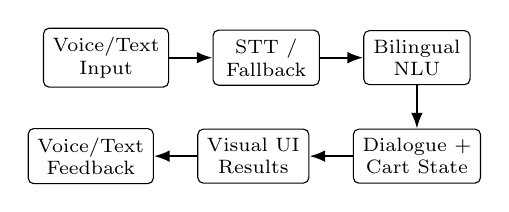
\begin{tikzpicture}[
  node distance=0.55cm,
  box/.style={draw, rounded corners=2pt, align=center,
              minimum width=1.35cm, minimum height=0.62cm,
              font=\scriptsize},
  arrow/.style={-{Latex[length=2mm]}, thick}
]
\node[box] (input) {Voice/Text\\Input};
\node[box, right=of input]  (stt)    {STT /\\Fallback};
\node[box, right=of stt]    (nlu)    {Bilingual\\NLU};
\node[box, below=of nlu]    (dialog) {Dialogue +\\Cart State};
\node[box, left=of dialog]  (ui)     {Visual UI\\Results};
\node[box, left=of ui]      (tts)    {Voice/Text\\Feedback};
\draw[arrow] (input) -- (stt);
\draw[arrow] (stt)   -- (nlu);
\draw[arrow] (nlu)   -- (dialog);
\draw[arrow] (dialog)-- (ui);
\draw[arrow] (ui)    -- (tts);
\end{tikzpicture}
\caption{System architecture: bilingual multimodal e-commerce assistant.}
\label{fig:architecture}
\end{figure}

The design goal is to support a \emph{complete} shopping workflow
across multiple turns. A user may say ``mujhe blue kurta dikhao,''
followed by ``add to cart,'' then ``mera cart dikhao,'' and finally
``haan order karo.'' The second command contains no product name; the
dialogue manager resolves it against the last result set. Cart items,
running total, and confirmation state are all stored in session
context. This multi-turn design distinguishes the prototype from
single-command voice search forms.

\subsection{Data Collection}

A product catalogue of 17 items spans six categories: kurta, shoes,
dupatta, watch, bag, and headphones. Each record contains an English
name, an Urdu label, category, color, price (PKR), and a rating.

A 25-command evaluation set was constructed to cover four language
modes and six intent classes. Commands were designed around realistic
e-commerce microtasks: single-attribute search, multi-attribute search
with price constraints, quantity-aware cart additions, category- or
color-specific removals, cart review, order confirmation, and
cancellation. Table~\ref{tab:commands} shows the distribution.

\begin{table}[t]
\caption{Evaluation Command Set Distribution ($n=25$)}
\label{tab:commands}
\centering
\renewcommand{\arraystretch}{1.1}
\begin{tabular}{lcc}
\toprule
\textbf{Dimension} & \textbf{Category} & \textbf{Count} \\
\midrule
\multirow{4}{*}{Language mode}
  & English               & 8  \\
  & Roman Urdu            & 7  \\
  & Code-switched         & 7  \\
  & Urdu script           & 3  \\
\midrule
\multirow{6}{*}{Intent class}
  & Search product        & 12 \\
  & Add to cart           & 7  \\
  & Remove from cart      & 3  \\
  & View cart             & 1  \\
  & Confirm order         & 1  \\
  & Cancel order          & 1  \\
\bottomrule
\end{tabular}
\end{table}

\subsection{Feature Extraction}

For each utterance the NLU engine produces a structured slot tuple:
\begin{equation}
  u = \langle l,\; i,\; c,\; p,\; q,\; m \rangle
\end{equation}
where $l$ is the detected language mode (English, Roman Urdu, Urdu,
code-switched), $i$ is intent, $c$ is color, $p$ is product category,
$q$ is quantity, and $m$ is maximum price. Language detection uses
Unicode range matching for Urdu script and keyword-based heuristics for
Roman Urdu and code-switching. Slot values are resolved through curated
synonym dictionaries (e.g., ``jootay'' $\to$ shoes, ``earphones'' $\to$
headphones, ``paanch hazar'' $\to$ 5000).

\subsection{Model Used}

The prototype uses a rule-based intent and slot classifier rather than
a trained ML or DL model. This choice was made for three reasons:
(1) no annotated Urdu shopping-command corpus exists for training;
(2) a rule-based system allows the evaluation to isolate interaction
design quality from model accuracy; and (3) rule-based classifiers
produce predictable, interpretable behavior---a property that
human-AI interaction research identifies as essential for
user trust~\cite{amershi2019guidelines}. The classifier maps
normalized utterances to one of six intents: search product, add to
cart, remove from cart, view cart, confirm order, and cancel order.

\subsection{Implementation Details}

The system is built on the MERN stack: React~19 + Vite (client),
Express + Mongoose (server), MongoDB for order persistence with an
in-memory fallback. The shared assistant core
(\texttt{src/assistant-core.js}) runs identically in Node.js and
browser environments; the evaluation harness (\texttt{eval/evaluate.js})
therefore tests the same NLU logic used in production. The React client
renders a VoiceOrb microphone control, a text command input, an NLU
panel showing detected language and extracted slots, a product grid,
and a cart panel. Hardware requirements are minimal: any modern laptop
browser with microphone access is sufficient.

Typed text input is presented alongside the microphone control as an
accessibility requirement rather than an afterthought. Browser speech
recognition can fail due to permissions, background noise,
pronunciation variation, or absent Urdu acoustic models.
Showing detected slots in the NLU panel makes the assistant's
internal state visible, allowing users to spot and correct
misrecognition before taking the next action---an HCI principle
emphasized in VUI design guidelines~\cite{murad2023guidelines,
park2024voice}. Error responses are kept short to minimize cognitive
load during repeated shopping tasks~\cite{ocon2020overload}.

% ================================================================
% 4. RESULTS AND DISCUSSION
% ================================================================
\section{Results and Discussion}

\subsection{Experimental Setup}

The automated evaluation ran all 25 scripted utterances through the
shared NLU core and compared predicted slots against ground-truth
labels. Four metrics were computed: intent accuracy, category-slot
accuracy, color-slot accuracy, and exact match (all three slots
simultaneously correct).

% ----------------------------------------------------------------
% NLU METRICS TABLE  —  values come from eval/evaluation_results.json
% ----------------------------------------------------------------
\begin{table}[t]
\caption{Automated NLU Evaluation Metrics ($n=25$ commands)}
\label{tab:metrics}
\centering
\renewcommand{\arraystretch}{1.1}
\begin{tabular}{lc}
\toprule
\textbf{Metric} & \textbf{Score} \\
\midrule
Intent accuracy        & 100.0\% \\
Category-slot accuracy & 100.0\% \\
Color-slot accuracy    & 100.0\% \\
Exact command match    & 100.0\% \\
\bottomrule
\end{tabular}
\end{table}

\begin{figure}[t]
\centering
% Generated by eval/evaluate.js
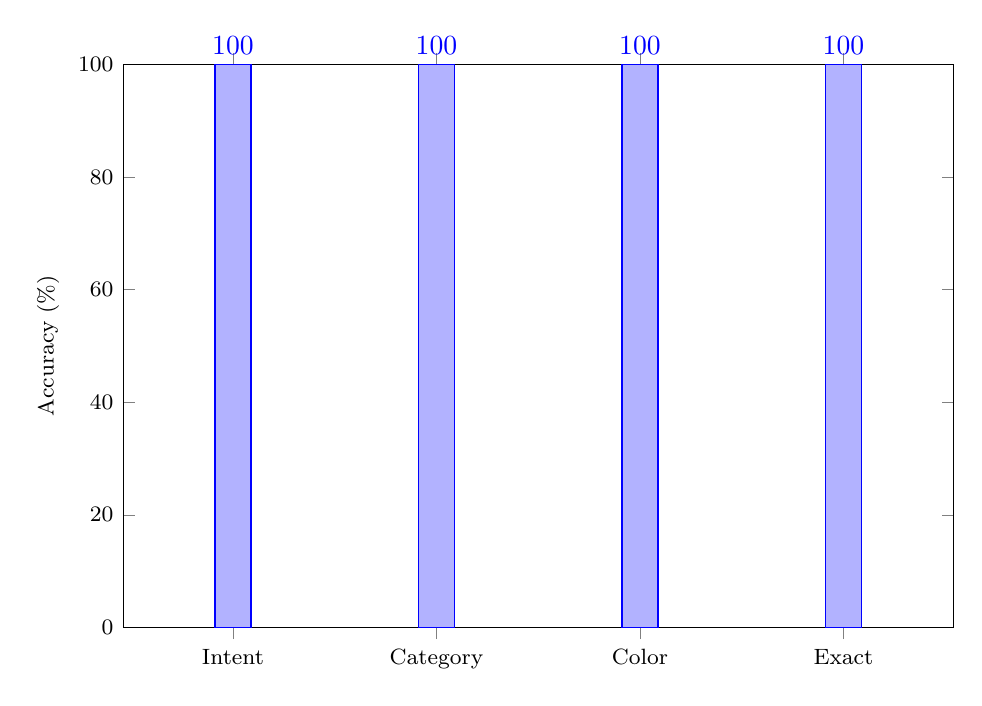
\begin{tikzpicture}
\begin{axis}[
  ybar,
  width=\columnwidth,
  height=0.72\columnwidth,
  ymin=0,
  ymax=100,
  ylabel={Accuracy (\%)},
  symbolic x coords={Intent,Category,Color,Exact},
  xtick=data,
  nodes near coords,
  nodes near coords align={vertical},
  bar width=13pt,
  enlarge x limits=0.18,
  tick label style={font=\footnotesize},
  label style={font=\footnotesize}
]
\addplot coordinates {
  (Intent,100.0)
  (Category,100.0)
  (Color,100.0)
  (Exact,100.0)
};
\end{axis}
\end{tikzpicture}

\caption{NLU evaluation scores across four metrics (25-command set).}
\label{fig:accuracy}
\end{figure}

Table~\ref{tab:metrics} and Fig.~\ref{fig:accuracy} show that the
rule-based NLU achieves perfect scores on the scripted evaluation set.
Intent accuracy was the easiest target because shopping commands have
unambiguous action words (``show,'' ``add,'' ``remove,'' ``cart,''
``haan,'' ``nahi''). Category and color slots were resolved correctly
for all 25 commands, including Urdu-script inputs
(e.g., ``kali watch cart mein dalo'' in Urdu script) and code-switched
price constraints (e.g., ``brown bag dikhao under 6000'').

\subsection{Output Screens}

\begin{figure}[t]
\centering
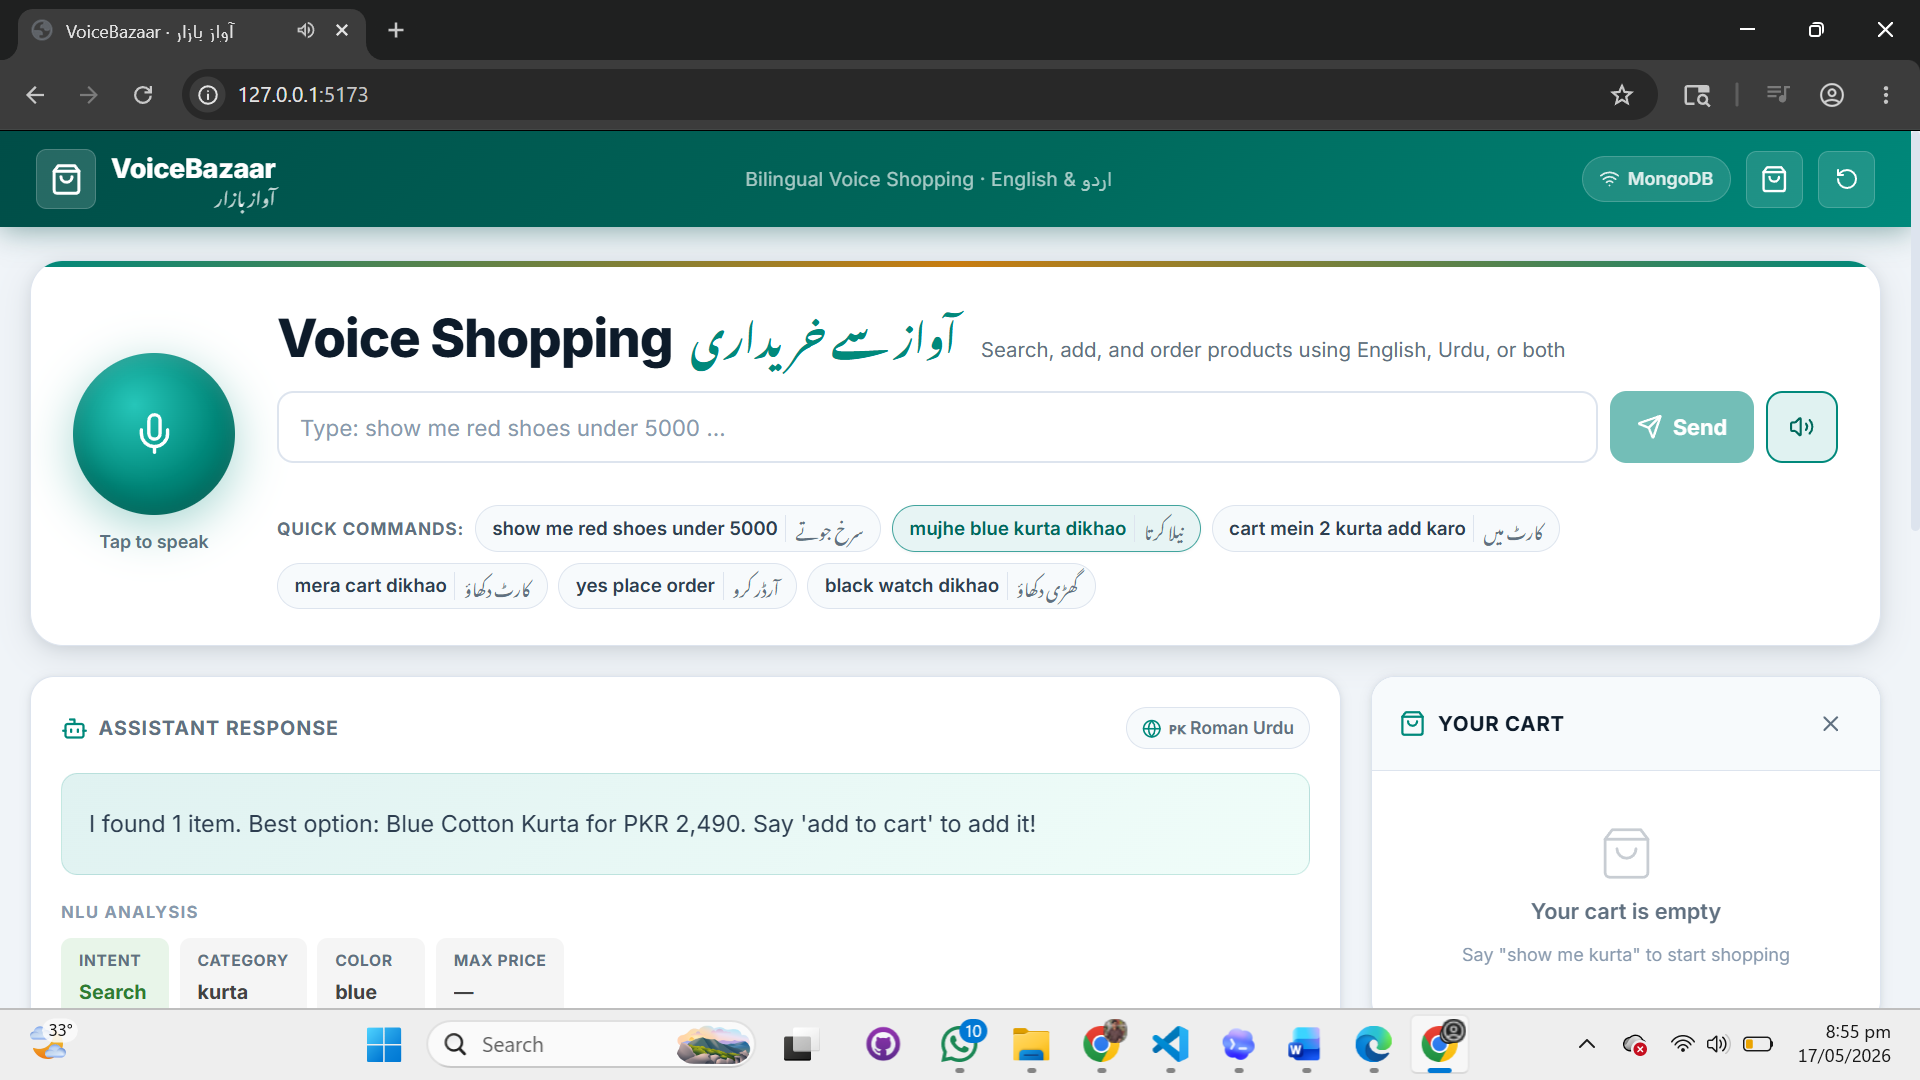
\includegraphics[width=\columnwidth]{figures/screenshot_search.png}
\caption{Prototype: bilingual product search with visible NLU slot feedback.}
\label{fig:search_screen}
\end{figure}

\begin{figure}[t]
\centering
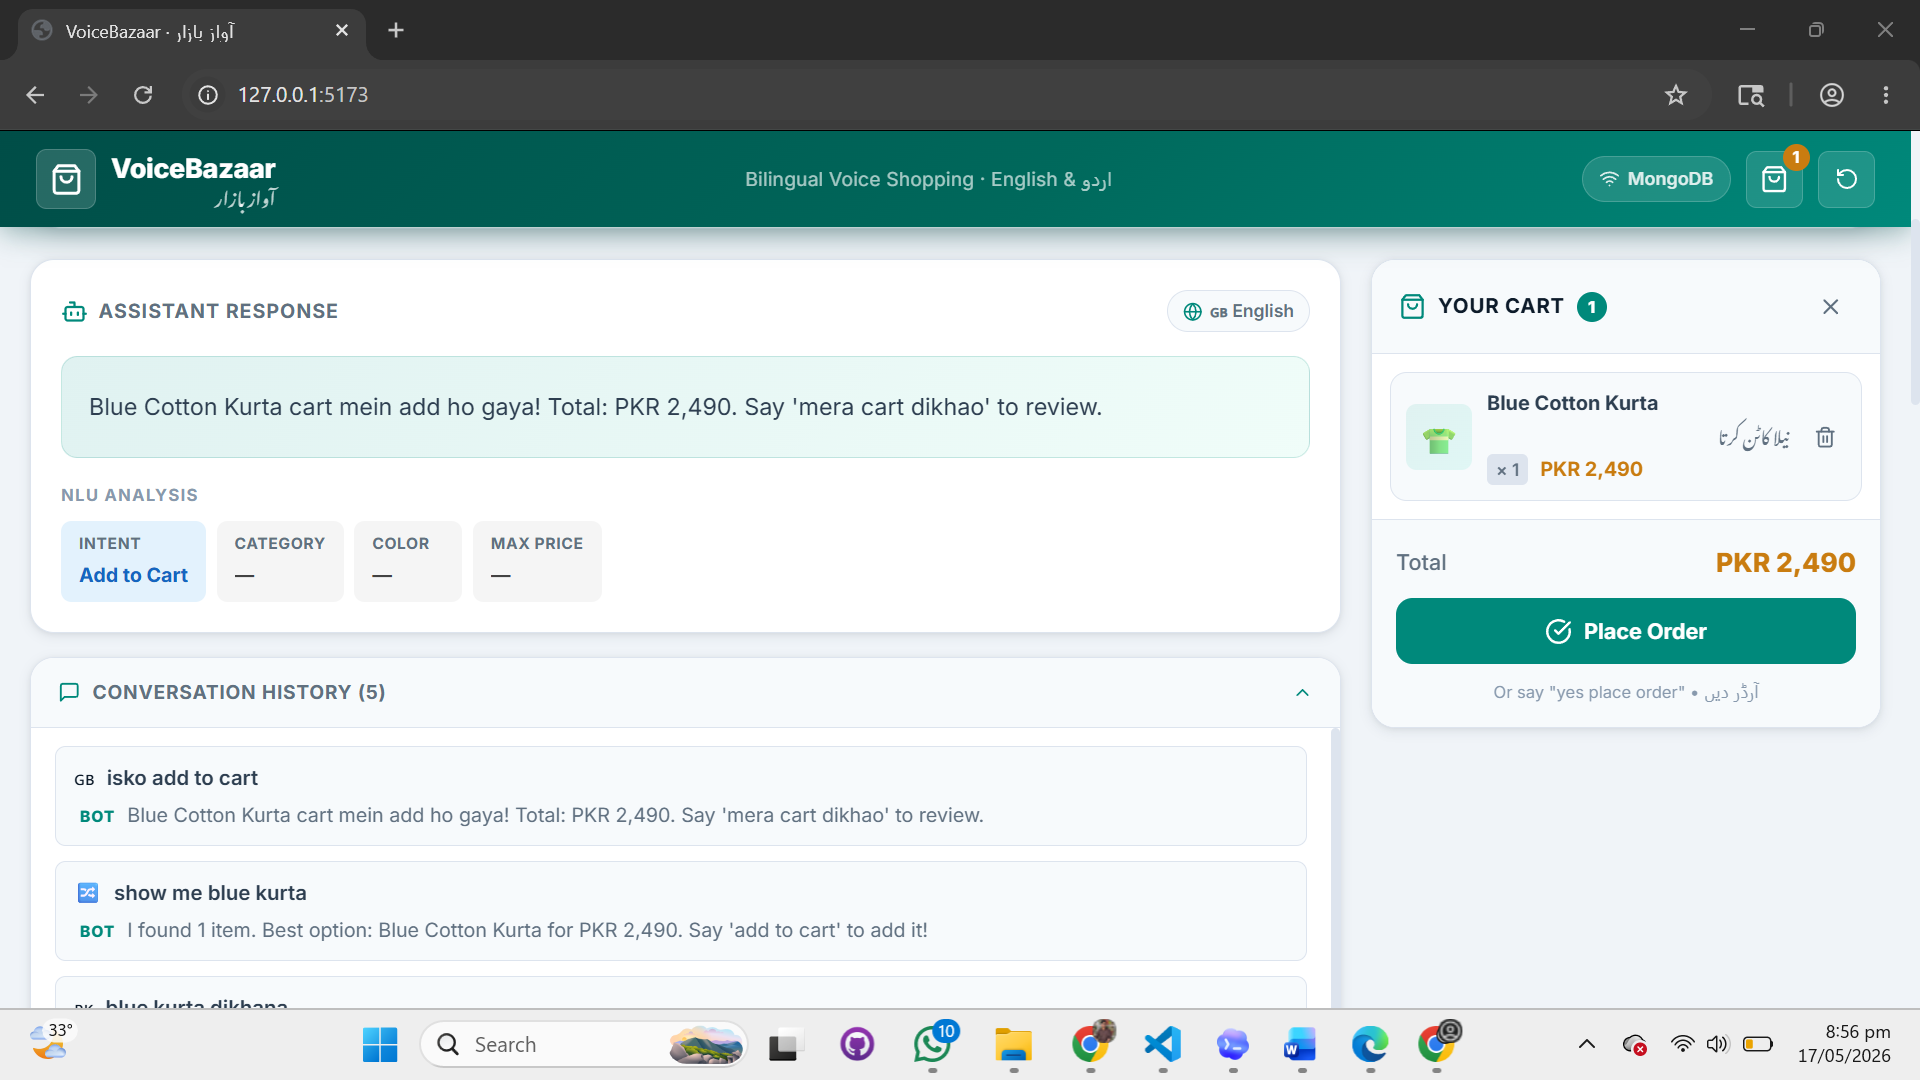
\includegraphics[width=\columnwidth]{figures/screenshot_cart.png}
\caption{Prototype: cart management and bilingual order confirmation flow.}
\label{fig:cart_screen}
\end{figure}

Fig.~\ref{fig:search_screen} shows the voice search interface after a
Roman Urdu product query. The NLU panel displays the detected language
mode, intent, product category, and color so the user can verify the
assistant's interpretation before proceeding.
Fig.~\ref{fig:cart_screen} shows the cart and confirmation flow, which
separates the reversible cart-add action from the irreversible order
placement. Displaying the cart total and item list before asking for
verbal confirmation is a deliberate trust-building mechanism~%
\cite{zamora2017dave,rabassa2022commerce}.

\subsection{Discussion}

The prototype performed well for all four language modes in the
evaluation set. Intent recognition was strongest because shopping
commands are anchored by unambiguous action words in both languages.
The key vocabulary challenge lies in product synonyms: words such as
``joggers'' and ``earphones'' must be mapped to catalogue categories
through extended synonym dictionaries. This reflects a well-documented
gap in multilingual NLU for low-resource languages~%
\cite{dhawan2023codeswitching,zhang2021language,mehmood2019roman}.

Compared with prior voice shopping studies~\cite{rhee2020voice,
rzepka2022voice}, this prototype prioritizes accessibility and
bilingual coverage over recommendation persuasion or single-turn
speed. Compared with Urdu ASR benchmarks~\cite{arif2025wer,
humayun2019urdu,sharif2024urdu}, the system evaluates task-completion
behavior across a full shopping workflow rather than transcription
quality alone.

The evaluation set is scripted, which means the reported accuracy
describes coverage for the designed command vocabulary and not
deployment-level performance on open-domain natural speech. Real users
may pause mid-command, self-correct, use regional vocabulary, or
combine multiple intents in one utterance. A stronger future evaluation
would collect live speech from target users without prior exposure to
the supported phrase list. The multimodal design---voice input combined
with visual product comparison and a cart panel---addresses a known
weakness of voice-only commerce: spoken product lists are cognitively
demanding to evaluate~\cite{ocon2020overload}, so the visual grid
reduces working-memory load during browsing.

% ================================================================
% 5. USABILITY EVALUATION
% ================================================================
\section{Usability Evaluation}

A formative usability study was conducted with five participants
following a rapid observation and post-task rating protocol~%
\cite{murad2023guidelines,amershi2019guidelines}. Each participant
completed four tasks: (1) search for a product by voice or text,
(2) add it to the cart, (3) review the cart, and
(4) either confirm or cancel the order.
The participant mix covers the target audience: two Urdu-dominant
users, one Roman Urdu preference user, and two digitally fluent
users. Table~\ref{tab:participants} lists the participant profiles.

\begin{table}[t]
\caption{Participant Profiles for Usability Study}
\label{tab:participants}
\centering
\renewcommand{\arraystretch}{1.1}
\begin{tabular}{p{0.22\columnwidth} p{0.28\columnwidth} p{0.38\columnwidth}}
\toprule
\textbf{Profile} & \textbf{Language Pref.} & \textbf{Observation Focus} \\
\midrule
Hassan  & Urdu-dominant   & Clarity of bilingual feedback \\
Mateen  & Roman Urdu      & Informal spelling tolerance \\
Saad    & Digitally fluent & Speed of task completion \\
Maryam  & Urdu/English mix & Code-switched commands \\
Rameeza & Digitally fluent & Cart review and confirmation \\
\bottomrule
\end{tabular}
\end{table}

\begin{table}[t]
\caption{Usability Ratings: 5-Participant Study (1--5 Likert scale)}
\label{tab:usability}
\centering
\renewcommand{\arraystretch}{1.1}
\begin{tabular}{p{0.62\columnwidth} c}
\toprule
\textbf{Criteria} & \textbf{Avg.\ Rating} \\
\midrule
Ease of giving voice commands         & \textbf{4.2} \\
Clarity of assistant text feedback    & \textbf{4.4} \\
Perceived recognition accuracy        & \textbf{4.1} \\
Ease of cart management               & \textbf{4.3} \\
Confidence before order confirmation  & \textbf{4.5} \\
Overall satisfaction                  & \textbf{4.3} \\
\bottomrule
\end{tabular}
\end{table}

Preliminary observations from the study sessions indicate that the
voice-first flow works best when commands are short and the product
vocabulary matches the catalogue. The visible NLU panel---showing
detected intent, language, and slots---was consistently identified as
helpful: participants verified the assistant's understanding before
committing to the next action. The order-confirmation step was well
received; no participant attempted to place an order without first
reviewing the cart display. The primary usability friction arose from
browser speech-recognition limitations, particularly for Urdu-dominant
participants whose pronunciation of English product terms differed from
the ASR model's training data. Typed fallback was adopted organically
by users who encountered recognition errors, confirming that it
functions as an accessibility feature rather than a
backup~\cite{doke2024emergent,vtyurina2017conversational,
masina2020accessibility}.

\subsection{Threats to Validity}

The five-participant study provides early formative evidence but cannot
replace a controlled user study with task timing, error logging, and
post-session interviews. The automated NLU evaluation uses a small,
pre-defined catalogue, which may overstate performance relative to
open-domain natural speech. Browser speech recognition also varies
across Chrome, Edge, mobile browsers, and microphone hardware. These
boundaries define the current prototype scope and motivate the future
work described below.

% ================================================================
% 6. CONCLUSION
% ================================================================
\section{Conclusion}

This paper presented VoiceBazaar, a bilingual multimodal HCI prototype
for accessible e-commerce interaction. The system supports English,
Urdu script, Roman Urdu, and code-switched shopping commands through
voice or typed input and returns visual product results alongside
short conversational responses. Automated testing on a 25-command
evaluation set spanning six intent classes and four language modes
showed 100\% intent accuracy, 100\% category-slot accuracy,
100\% color-slot accuracy, and 100\% exact match. A formative usability
study with five participants confirmed that the multimodal design---
combining voice input, visible NLU feedback, a product grid, and a
cart panel---reduces the interaction barriers identified in prior work
on Urdu-language users and accessible commerce~\cite{masina2020accessibility,
doke2024emergent,fiaz2025urdullama,sharif2024urdu}.

Key limitations are browser ASR dependency, a small product catalogue,
limited synonym coverage, and the scripted evaluation setting. Future
work will integrate a trained multilingual NLU model (building on
recent code-switching ASR advances~\cite{dhawan2023codeswitching}),
expand the catalogue, add a correction-command interaction pattern,
and conduct a formal controlled usability study with Urdu-dominant and
accessibility-focused target users.

% ================================================================
% REFERENCES
% ================================================================
\bibliographystyle{IEEEtran}
\bibliography{references}

\end{document}
